\documentclass[preprint,12pt]{elsarticle}
\usepackage[T1]{fontenc}
\usepackage[utf8]{inputenc}
\usepackage[cyr]{aeguill}
\usepackage[english]{babel}
\usepackage{amsmath,amssymb,amsthm}
\usepackage{bm}
\usepackage{graphicx}

\usepackage{natbib}
	
\usepackage[colorlinks=true,linkcolor=black, citecolor=blue, urlcolor=blue]{hyperref}

\usepackage{comment}
\usepackage{geometry}
\geometry{top=2cm,bottom=2.5cm,left=2.5cm,right=2.5cm}

\usepackage{mathrsfs}

\newcommand{\tens}[1]{%
	\mathbin{\mathop{\otimes}\displaylimits_{#1}}%
}

%\usepackage{hyperref}

\DeclareMathOperator*{\argmax}{arg\,max}
\DeclareMathOperator*{\argmin}{arg\,min}
\DeclareMathOperator{\Tr}{Tr}

\usepackage{diffcoeff}

\newtheorem{theorem}{Theorem}
\newtheorem{remark}{Remark}
\newtheorem{proposition}{Proposition}


\graphicspath{{./Figures/}}

\newcommand{\matr}[1]{\bm{#1}} 

\def\onedot{$\mathsurround0pt\ldotp$}
\def\cddot{% two dots stacked vertically
	\mathbin{\vcenter{\baselineskip.67ex
			\hbox{\onedot}\hbox{\onedot}}%
}}

\makeatletter \renewcommand\d[1]{\ensuremath{%
  \;\mathrm{d}#1\@ifnextchar\d{\!}{}}}
\makeatother

\journal{Elsevier}

\begin{document}
	
	\begin{frontmatter}	
		%% Title, authors and addresses
		
		%% use the tnoteref command within \title for footnotes;
		%% use the tnotetext command for theassociated footnote;
		%% use the fnref command within \author or \address for footnotes;
		%% use the fntext command for theassociated footnote;
		%% use the corref command within \author for corresponding author footnotes;
		%% use the cortext command for theassociated footnote;
		%% use the ead command for the email address,
		%% and the form \ead[url] for the home page:
		%% \title{Title\tnoteref{label1}}
		%% \tnotetext[label1]{}
		%% \author{Name\corref{cor1}\fnref{label2}}
		%% \ead{email address}
		%% \ead[url]{home page}
		%% \fntext[label2]{}
		%% \cortext[cor1]{}
		%% \address{Address\fnref{label3}}
		%% \fntext[label3]{}	
		\title{Port-Hamiltonian formulation and \\
		Symplectic discretization of plate models\\
		\vspace{2mm} \large\textit{Part II : Kirchhoff model for thin plate}}	
		%% use optional labels to link authors explicitly to addresses:
		%% \author[label1,label2]{}
		%% \address[label1]{}
		%% \address[label2]{}
		\author[ISAE]{Andrea Brugnoli\corref{cor1}}
		\ead{Andrea.Brugnoli@isae.fr}
		
		\author[ISAE]{Daniel Alazard}
		\ead{Daniel.Alazard@isae.fr}
		
		\author[ISAE]{Valérie Pommier-Budinger}
		\ead{Valerie.Budinger@isae.fr}
		
		\author[ISAE]{Denis Matignon}
		\ead{Denis.Matignon@isae.fr}
		
		\cortext[cor1]{Corresponding author}
		
		
	    \address[ISAE]{ISAE-SUPAERO, Université de Toulouse, France.\\
		\vspace{2mm} {10 Avenue Edouard Belin, BP-54032, 31055 Toulouse Cedex 4.}}
		
		\begin{abstract}
		The mechanical model of a thin plate with boundary control and 
        observation is presented as a port-Hamiltonian system (pHs\footnote{pHs stands for port-Hamiltonian systems.}), both in vectorial and tensorial forms: the Kirchhoff-Love model of a plate is described by using a Stokes-Dirac structure and this represents a novelty with respect to the existing literature. This formulation is carried out both in vectorial and tensorial forms. Thanks to tensorial calculus, this model is found to mimic the interconnection structure of its one-dimensional counterpart, i.e. the Euler-Bernoulli beam. \\
        The Partitioned Finite Element Method (PFEM\footnote{PFEM stands for partitioned finite element method.}) is then extended to obtain a suitable, i.e. structure-preserving, weak form. The discretization procedure, performed on the vectorial formulation, leads to a finite-dimensional port-Hamiltonian system.  This part II of the companion paper extends part I, dedicated to the Mindlin model for thick plates. The thin plate model comes along with additional difficulties, because of the higher order of the differential operator under consideration.
		\end{abstract}
		
		\begin{keyword}
			%% keywords here, in the form: keyword \sep keyword
			%% PACS codes here, in the form: \PACS code \sep code
			%% MSC codes here, in the form: \MSC code \sep code
			%% or \MSC[2008] code \sep code (2000 is the default)
			port-Hamiltonian systems	 \sep Kirchhoff plate \sep Partitioned Finite Element Method \sep geometric spatial discretization \sep boundary control.
		\end{keyword}
	
	
   
	\end{frontmatter}
	
	
\section*{Introduction}
As presented in part I of this companion paper, the port-Hamiltonian (PH) formalism \cite{BookZwart, bookPHs, Villegas} allows the structured modeling and discretization of multi-physics applications involving interconnected finite- and infinite-dimensional systems (\cite{Cervera2007,ShaftIntInfinite,vanderShaftintFinInf}). Preserving the port-Hamiltonian structure in the discretization process is a keypoint to take benefit of this powerful formalism. This issue was fisrt addressed in \cite{Golo}, with a mixed finite element spatial discretization method, and in \cite{moulla:hal-01625008}, with pseudo-spectral methods relying on higher-order global polynomial approximations. All those methods are difficult to implement, especially for those system the spatial dimension of which is bigger than one. Very recently weak formulations which lead to Galerkin numerical approximations began to be explored: in \cite{WeakForm_Kot}, a structure preserving finite element method was introduced for the wave equation in a two-dimensional domain; this method exhibits good results, both in the spectral analysis and simulation part, though requiring of a primal and a dual mesh on the geometry of the problem. Another approach is the partitioned finite element method (PFEM) proposed in \cite{LHMNLCFlavio2018}, already largely explored in part I of this companion paper; the advantages of this latter methodology are its simplicity of implementation and its potential to carry over to a wide set of examples, no matter the spatial dimension of the problem; the possible use of open source software like FreeFEM++ or FEniCS is also an appealing feature of this latter method  \\

In part II of this companion paper, the modeling and discretization of thin plates described by the Kirchhoff-Love plate model is carried out within the PH framework, allowing for boundary control and observation. Compared to the existing literature on either the symplectic Hamiltonian formulation of  \cite{LI2016984,LI2018310}, or the port-Hamiltonian framework throgh jet theory in \cite{SchobertMindlin,SCHOBERL2015610}, the main contribution of this paper concerns the PH formalism based on a Stokes-Dirac structure. This formalism is presented both in vectorial and tensorial forms.  Moreover, the tensorial formalism \cite[Chapter~16]{Grinfield} highlights that this model mimics the interconnection structure of its one-dimensional counterpart, i.e. the Euler-Bernoulli beam. Compared to part I dedicated to thick plate Mindlin model in which first-order differential operators are explored in dimension two, and compared to \cite{LeGorrec2005} in which second-  or higher-order differential operators were explored in dimension one only, the contribution of this paper is the PH formalism of systems of dimension two described with second-order  differential operators, such as the Kirchhoff-Love  model. 
The model, once written in a tensorial form, highlights new insights on second-order differential operators: especially the double divergence and the Hessian are proved to be adjoint operators one of another, which represents another important contribution of this paper.
Finally, the extension of the PFEM method  to the structure-preserving discretization of the Kirchhoff model  is also a novelty of the paper. It allows simple implementation of numerical schemes compared to the jet theory formalism, while preserving the structure of PHS at the discrete level. 

\section{Second-order distributed PH systems: Euler-Bernoulli beam}	
The Euler-Bernoulli beam is the one-dimensional equivalent of the Kirchhoff-Love plate. The reader can refer to \cite{Gorrec2017} for a stability proof of a beam connected to non linear springs and dampers or to \cite{aoues:hal-01738092} for an illustration of rotating spacecraft with flexible appendages model as PH Bernoulli beams. This model consists of one PDE, describing the vertical displacement along the beam length
\begin{equation}
\rho(x) \diffp[2]{w}{t}(x,t) + \displaystyle \diffp[2]{}{x} \left( EI(x) \diffp[2]{w}{x} \right) = 0, \quad x \in (0,L),\, t \ge 0 
\end{equation}
where ${w}(x,t)$ is the transverse displacement of the beam. The coefficients $\rho(x), E(x)$ and $I(x)$  are the mass per unit length, Young's modulus of elasticity and the moment of inertia of a cross section. The energy variables are then chosen as follows
\begin{equation}
\begin{aligned}
\alpha_{w} &= \rho(x) \diffp{w}{t}(x,t),  \quad \text{Linear Momentum},\\
\alpha_{\kappa} &= \diffp[2]{w}{x}(x,t), \quad \text{Curvature}. \\
\end{aligned}
\end{equation}

Those variables are collected in the vector $\bm{\alpha} = (\alpha_{w}, \, \alpha_{\kappa})^T $, so that the Hamiltonian can be written as a quadratic functional in the energy variables 
\begin{equation}
H = \frac{1}{2} \int_{0}^{L} \bm{\alpha}^T Q \bm{\alpha} \; \d{x},
\qquad \text{where} \qquad
Q = 
\begin{bmatrix}
\frac{1}{\rho(x)} & 0 \\
0 & EI(x) \\
\end{bmatrix}.
\end{equation}

The co-energy variables are found by computing the variational derivative of the Hamiltonian
\begin{equation}
\begin{aligned}
e_{w} &:= \diffd{H}{\alpha_w} = \diffp{w}{t}(x,t) ,  \quad \text{Vertical velocity}, \\
e_{\kappa} &:= \diffd{H}{\alpha_{\kappa}} =EI(x) \diffp[2]{w}{x}(x,t),  \quad \text{Flexural momentum}. \\
\end{aligned}
\end{equation}
Those variables are again collected in vector $\bm{e} = (e_{w}, \, e_{\\kappa})^T $, so that the underlying interconnection structure is then found to be
\begin{equation}
\label{eq:PH_Timo}
\diffp{\bm{\alpha}}{t} = J \mathbf{e},  	\qquad \text{where} \qquad
J = 
\begin{bmatrix}
0 & -\diffp[2]{}{x} \\
\diffp[2]{}{x} & 0 \\
\end{bmatrix}.
\end{equation}

For an infinite-dimensional system, boundary variables have to be defined as well. Those can be found by evaluating the energy rate flow across the boundary. One possible choice among others (see \cite{articleFlavio} for a more exhaustive explanation) for this model is the following 

\begin{equation}
\bm{f}_{\partial} = 
\begin{pmatrix}
e_w(0) \vspace{3pt} \\
\displaystyle \diffp{e_{w}}{x}(0) \vspace{3pt}\\
\displaystyle \diffp{e_{\kappa}}{x}(L) \vspace{3pt}\\
e_{\kappa}(L) \\
\end{pmatrix}, \qquad
\bm{e}_{\partial} = 
\begin{pmatrix}
\displaystyle \diffp{e_{\kappa}}{x}(0) \vspace{1pt}\\
-e_{\kappa}(0) \\
-e_w(L) \\
\displaystyle \diffp{e_{w}}{x}(L)\\
\end{pmatrix}.
\end{equation}
The power flow is then easily evaluated as
\begin{equation}
\frac{d}{dt} H(t) = \int_{0}^{L} \diffp{\bm{\alpha}}{t} \cdot \bm{e} \, \d{x} = \left\langle \bm{e}_{\partial}, \bm{f}_{\partial} \right\rangle_{{\rm I\!R}^4}.
\end{equation}

The flow variables can now be defined as $\bm{f} = - \diffp{\bm{\alpha}}{t}$, so that the flow space is given by the tuples
$(\bm{f},\bm{f}_{\partial}) \in \mathcal{F}$. Equivalently the effort space is given by $(\bm{e},\bm{e}_{\partial}) \in \mathcal{E}$. The bond space is therefore the Cartesian product of the two
\begin{equation}
\mathcal{B} := \left\{(\bm{f},\bm{f}_{\partial},\bm{e},\bm{e}_{\partial}) \in \mathcal{F} \times \mathcal{E} \right\}.
\end{equation}

The duality pairing between elements of $\mathcal{B}$ is then defined as follows
\begin{equation}
\label{eq:bil_Timo}
\ll ((\bm{f}^a,\bm{f}_{\partial}^a), (\bm{e}^a,\bm{e}_{\partial}^a)), ((\bm{f}^b,\bm{f}_{\partial}^b), (\bm{e}^b,\bm{e}_{\partial}^b)) \gg := \int_{0}^{L}\left\{ (\bm{f}^{a})^T \bm{e}^b + (\bm{f}^{b})^T \bm{e}^a \right\} \d{x} + (\bm{f}_{\partial}^{a})^T \bm{e}_{\partial}^b + (\bm{f}_{\partial}^{b}) ^T \bm{f}_{\partial}^a.
\end{equation}
The Stokes-Dirac structure for the Euler-Bernoulli beam is therefore the following
\begin{theorem}[From \cite{LeGorrec2005}, Stokes-Dirac structure for the Bernoulli beam]
	Consider the space of power variables $\mathcal{F} \times \mathcal{E}$= and the bilinear form (+pairing operator) $\ll , \gg$ given by \eqref{eq:bil_Timo}. Define the following linear subspace $\mathcal{D} \subset \mathcal{F} \times \mathcal{E}$
	\begin{equation}
	\mathcal{D} =  \left\{(\bm{f},\bm{f}_{\partial},\bm{e},\bm{e}_{\partial}) \in \mathcal{F} \times \mathcal{E} | \; \bm{f} = -J\bm{e},  \quad
	\begin{aligned}
	\bm{f}_{\partial} &= 
	\begin{pmatrix} 
	e_w(0) \vspace{3pt} & \displaystyle  \diffp{e_{w}}{x}(0) & \displaystyle \diffp{e_{\kappa}}{x}(L) &	e_{\kappa}(L) \\
	\end{pmatrix}^T \\
	\bm{e}_{\partial} &= 
	\begin{pmatrix}
	\displaystyle \diffp{e_{\kappa}}{x}(0) & 	-e_{\kappa}(0) & -e_w(L) & \displaystyle \diffp{e_{w}}{x}(L)\\
	\end{pmatrix}^T
	\end{aligned} \right\}.
	\end{equation}
	Then $\mathcal{D} = \mathcal{D}^{\perp}$, where $\mathcal{D}^{\perp}$ is understood in the sense of orthogonality wit respect to the bilinear product $\ll , \gg$  i.e $\mathcal{D}$ is a Dirac structure. 
\end{theorem}

	\section{Kirchhoff-Love theory for thin plates}
	In this section the classical variational approach (Hamilton's principle) to derive the equation of motions is first detailed. The physical quantities involved and the different energies, of utmost importance for the PH formalism, are reminded.
	
	
	\subsection{Model and associated variational formulation}
	\label{sec:VarKir}
	The Kirchhoff-Love plate formulation rests on the hypothesis of small thickness compared to the in plane dimensions. The notations and symbols are borrowed form \cite{FEM_Cook} and \cite{Oslo}. The displacement field and the strains are defined by assuming that fibers orthogonal to the middle plane remain orthogonal (see figure \ref{fig:Kirchh_sketch}). This leads to the following relations for the displacement field 
	\begin{equation}
	u(x,y,z) = -z \diffp{w}{x}, \qquad v(x,y,z) = -z \diffp{w}{y}, \qquad 
	w(x,y,z) = w(x,y).
	\end{equation}
	and for the strains
	\begin{equation}
	\bm{\epsilon} =  
	\begin{pmatrix}
	\epsilon_{xx} \\
	\epsilon_{yy} \\
	\gamma_{xy} \\
	\end{pmatrix}  = 
	\begin{pmatrix}
	\diffp{}{x} & 0 \\
	0 & \diffp{}{y} \\
	\diffp{}{y} & \diffp{}{x} \\
	\end{pmatrix}
	\begin{pmatrix}
	-z \diffp{w}{x}\\
	-z \diffp{w}{y}\\
	\end{pmatrix} = 
	-z
	\begin{pmatrix}
	\diffp[2]{w}{x} \\
	\diffp[2]{w}{y} \\
	2 \diffp{w}{x,y} \\
	\end{pmatrix}. 
	\end{equation}
The curvature vector is defined as	
\begin{equation}
	\bm{\kappa} = 
\begin{pmatrix}
\kappa_{xx} \\
\kappa_{yy} \\
\kappa_{xy} \\
\end{pmatrix} = 
\begin{pmatrix}
\diffp[2]{w}{x} \\
\diffp[2]{w}{y} \\
2 \diffp{w}{x,y} \\
\end{pmatrix}.
\end{equation}

	\begin{figure}[tb]
		\centering
		\includegraphics[width=0.8\textwidth]{Kirchh_sketch.eps}
		\caption{Kinematic assumption for the Kirchhoff plate}
		\label{fig:Kirchh_sketch}
	\end{figure}
	
	The Hooke constitutive law for isotropic material is considered for the constitutive relation
	\begin{equation}
	\bm{\sigma} = 
	\bm{E} \bm{\epsilon} , \qquad \bm{E} :=
	\frac{E}{1 - \nu^2}
	\begin{bmatrix}
	1 & \nu & 0 \\
	\nu & 1 & 0 \\
	0  &  0 & \frac{1-\nu}{2}\\
	\end{bmatrix}.
	\end{equation}
	where $\nu$ the Poisson ratio and $E$ the Young modulus.
	The generalized momenta are found by integrating the stresses along the fiber
	\begin{equation*}
	\bm{M} =
	\begin{pmatrix}
	M_{xx} \\
	M_{yy} \\
	M_{xy} \\
	\end{pmatrix} = \int_{-\frac{h}{2} }^{\frac{h}{2}}
	-z \bm{\sigma} \d{z}=
	\left( \int_{-\frac{h}{2} }^{\frac{h}{2}}
	\bm{E} z^2 \d{z} \right) \bm{\kappa}
	\end{equation*}
	
	If it is assumed that the mechanical properties remain constant along the $z-$axis, then momenta are expressed vectorially as follows 
	\begin{equation}
	\bm{M}=
	\begin{pmatrix}
	M_{xx} \\
	M_{yy} \\
	M_{xy} \\
	\end{pmatrix} = 
	\begin{pmatrix}
	D\left(\diffp[2]{w}{x} + \nu \diffp[2]{w}{y}\right)\\
	D\left(\diffp[2]{w}{y} + \nu \diffp[2]{w}{x}\right)\\
	D (1 - \nu) \diffp{w}{x,y} \\
	\end{pmatrix}.
	\end{equation}
	where  $D = \frac{E h^3}{12 (1 - \nu^2)}$ is the bending rigidity and, in the most general case, $D = D(x,y), \; \nu = \nu(x,y)$. The relation between momenta and curvatures is expressed by matrix $\bm{D}$:
	\begin{equation}
	\mathbf{M} = \matr{D} \bm{\kappa}, \qquad 
	\matr{D} := 
	\int_{-\frac{h}{2} }^{\frac{h}{2}}
	\bm{E} z^2 \d{z} = D 
	\begin{bmatrix}
	1 & \nu & 0 \\ 
	\nu & 1 & 0 \\
	0    & 0 & \frac{1}{2} (1 - \nu)
	\end{bmatrix}.
	\end{equation}
	
	The Kirchhoff-Love model arises as the Euler-Lagrange equation stemming from the following extrema problem (Hamilton principle):
	
	\begin{equation*} 
	w_0 = \{w \in \mathcal V; \; \left.\delta F(w) \right|_{w_0} = 0\}
	\end{equation*}
	and
	\begin{multline*}
	F(w) = \int_0^T \int_\Omega \left\{\mathcal{K} - \mathcal{U} + \mathcal{W} \right\} \d{\Omega} \, \d{t} = \int_0^T \int_\Omega \left\{\frac{1}{2} \mu \left(\diffp{w}{t}\right)^2 - \frac{1}{2} D \left[ \left(\diffp[2]{w}{x}\right)^2 \right. \right. + \\
	\left. + \left(\diffp[2]{w}{y}\right)^2 + 2\nu
	\left(\diffp[2]{w}{x}\right) \left(\diffp[2]{w}{y}\right)  \left. + 2 (1 - \nu) \left(\diffp{w}{x,y} \right)^2 \right] + p w \right\} \d{\Omega} \, \d{t},
	\end{multline*}
	
	where $\mu$ the surface density, $p(x,y)$ the vertical load density. For example if gravity along the $z$ axis is considered $p = -\mu g$. The domain $\Omega$ is a connected region of $\mathbb{R}^2$. Furthermore, $\mathcal{V}$ is a suitable functional space, which contains the essential boundary conditions, i.e. Dirichlet conditions; as usual, Neumann boundary conditions will be specified by means of the variational problem itself. This formulation is not complete since boundary terms may be added to take into account non homogeneous boundary conditions. Moreover, the external work $\mathcal{W}$, $\mathcal{K}$ and $\mathcal{U}$, the kinetic and potential energy density per unit area, are respectively given by
	
	\begin{align*}
	\mathcal{W} &= pw, \\
	\mathcal{K} &= \frac{1}{2} \mu \left(\diffp{w}{t}\right)^2,\\
	\mathcal{U} &= \frac{1}{2} D \left[ \left(\diffp[2]{w}{x} \right)^2 + \left(\diffp[2]{w}{y}\right)^2 
	+ 2\nu \left(\diffp[2]{w}{x}\right) \left(\diffp[2]{w}{y}\right)  \  + 2 (1 - \nu) \left(\diffp{w}{x,y}\right)^2 \right], \\
	&= \frac{1}{2} \bm{\kappa}^T \matr{D} \bm{\kappa} \, .	
	\end{align*} 
	
	The total energy density is split into kinetic and potential energy
	\begin{equation}
	\mathcal{H} = \mathcal{K} + \mathcal{U},
	\end{equation}
	and the corresponding total energies given by the following relations
	\begin{equation}
	H = \int_{\Omega} \mathcal{H} \ \d{\Omega}, \qquad K = \int_{\Omega} \mathcal{K} \ \d{\Omega}, \qquad U = \int_{\Omega} \mathcal{U} \ \d{\Omega}.
	\end{equation}
	The Euler-Lagrange equation reads
	\begin{equation}
	\mu \diffp[2]{w}{t}  + \diffp[2]{M_{xx}}{x} + 2 \diffp{M_{xy}}{x,y} + \diffp[2]{M_{yy}}{y}= p.
	\end{equation}
	The spatial derivatives of the acceleration have been neglected. If the $D, \nu$ coefficients are constant then the ruling EDP becomes
	\begin{equation}
	\mu \diffp[2]{w}{t}  + D \Delta^2 w= p ,
	\end{equation}
	where $\Delta^2 = \diffp[4]{}{x} + 2 \diffp[2,2]{}{x,y} + \diffp[4]{}{y}$ is the bilaplacian. In the sequel it is assumed $p =0$.
	The specification of boundary conditions allows defining the function space $\mathcal{V}$. 
	
	\section{PH formulation of the Kirchhoff plate}
	In this section the port-Hamiltonian formulation of the Kirchhoff plate is presented first in vectorial form  in \ref{sec:PH_vec_Kir} and then in tensorial form in \ref{sec:PH_ten_Kir}.
	
	\subsection{PH vectorial formulation of the Kirchhoff plate}
	\label{sec:PH_vec_Kir}
	
	To obtain a port-Hamiltonian system (pHs) the energy variables as well as the underlying Stokes-Dirac structure, associated with the skew-adjoint operator $J$, have to be properly defined. Since the Kirchhoff plate represents the 2D extension of the Euler-Bernoulli beam, it is natural to select as energy variables the linear momentum, together with curvatures. The energy variables are collected in the vector
	\begin{equation}
	\bm{\alpha} := (\mu v,\ \kappa_{xx},\ \kappa_{yy},\ \kappa_{xy})^T,
	\end{equation}
	where $v = \diffp{w}{t}$. The Hamiltonian density is given by the following expression
	\begin{equation}
	\label{eq:H_kir}
	\mathcal{H} = \frac{1}{2} \bm{\alpha}^T \begin{bmatrix}
	\frac{1}{\mu} & 0 \\
	0 & \bm{D} \\
	\end{bmatrix} \bm{\alpha},  \qquad H = \int_{\Omega} \mathcal{H} \ \d{\Omega}.
	\end{equation}
	So its variational derivative provides as co-energy variables
	\begin{equation}
	\mathbf{e} := \diffd{H}{\bm{\alpha}} = (v,\ M_{xx},\ M_{yy},\ M_{xy})^T,
	\end{equation}
	The port-Hamiltonian system and the formally skew-adjoint operator relating energy and co-energy variables are found to be
	\begin{equation}
	\label{eq:PH_Kirchh}
	\diffp{\bm{\alpha}}{t} = J \mathbf{e} \quad \text{and} \quad J := 
	\begin{bmatrix}
	0 & -\diffp[2]{}{x} & -\diffp[2]{}{y} & - \left(\diffp{}{x,y} + \diffp{}{y,x} \right)\\
	\diffp[2]{}{x} & 0 & 0 & 0 \\
	\diffp[2]{}{y} & 0 & 0 & 0 \\
	\diffp{}{x,y} +  \diffp{}{y,x} & 0 & 0 & 0 \\
	\end{bmatrix}.
	\end{equation}
	\begin{remark}
		From the Schwarz theorem for $C^2$ functions the mixed derivative could be be expressed as $2 \diffp{}{x,y}$, instead of $\diffp{}{y,x} + \diffp{}{x,y}$. However, in this way the symmetry intrinsically present in $\gamma_{xy} = -z \left( \diffp{w}{y,x} + \diffp{w}{x,y} \right)$ would be lost. The mixed derivative is here split to reestablish the symmetric nature of curvatures and momenta (that are of tensorial nature as explained in section \ref{sec:PH_ten_Kir}).
	\end{remark}
	The boundary variables are obtained by evaluating the time derivative of the Hamiltonian
	\begin{align*}
	\dot{H} &= \int_\Omega \diffd{H}{\bm{\alpha}}   \cdot \diffp{\bm{\alpha}}{t} \; \d{\Omega} \\
	&= \int_\Omega \left\{ v \left(-\diffp[2]{M_{xx}}{x} -\diffp[2]{M_{xx}}{y} - 2 \diffp{M_{xy}}{x,y} \right) + M_{xx} \diffp[2]{v}{x} + M_{yy} \diffp[2]{v}{y} + 2 M_{xy} \diffp{v}{x,y} \right\} \d{\Omega} \\
	&= \int_\Omega \left\{ e_1 \left(-\diffp[2]{e_2}{x} -\diffp[2]{e_3}{y} - 2 \diffp{e_4}{x,y}\right) + e_2 \diffp[2]{e_1}{x} + e_3 \diffp[2]{e_1}{y} + 2 e_4 \diffp{e_1}{x,y}  \right\} \d{\Omega}
	\end{align*}
	
	\begin{figure}[t]
		\centering
		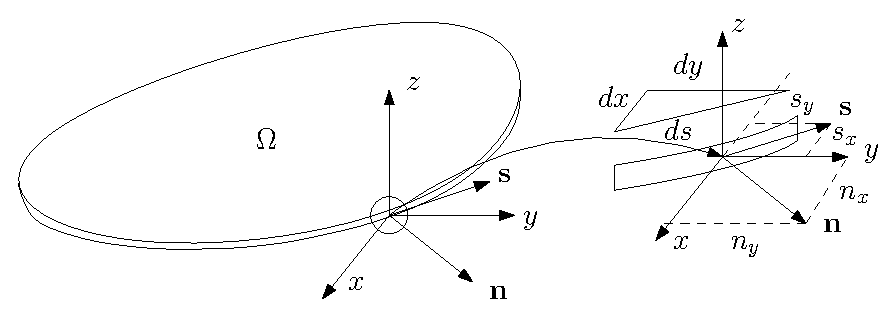
\includegraphics[height=0.2\textheight]{Plate_ref.eps}
		\caption{Reference frames and notations}
		\label{fig:plate_ref}
	\end{figure}
	
	In Figure \ref{fig:plate_ref} the notations for the different reference frames are introduced. By applying Green theorem, considering the split mixed derivative ($2 \diffp{}{x,y} = \diffp{}{x,y} +  \diffp{}{y,x}$)
	
	\begin{comment}
	\begin{equation}
	\label{Hdot1}
	\dot{H} = \int_{\partial \Omega} \left\{ n_x \left(e_2 \diffp{e_1}{x} - e_1 \diffp{e_2}{x} + 2 e_4 \diffp{e_1}{y} \right) + n_y \left(e_3 \diffp{e_1}{y} - e_1 \diffp{e_3}{y} - 2 e_1 \diffp{e_4}{x} \right) \right\} \d{s}
	\end{equation}
	Or, equivalently, 
	\begin{equation}
	\label{Hdot2}
	\dot{H} = \int_{\partial \Omega} \left\{ n_x \left(e_2 \diffp{e_1}{x} - e_1 \diffp{e_2}{x} - 2 e_1 \diffp{e_4}{y}\right) + n_y \left(e_3 \diffp{e_1}{y} - e_1 \diffp{e_3}{y} + 2 e_4 \diffp{e_1}{x}\right) \right\} ds
	\end{equation}
	The half-sum of equations \eqref{Hdot1}, \eqref{Hdot2} does restore symmetry
	\end{comment} 

	\begin{align}
	\dot{H} = \int_{\partial \Omega}  & \left\{  n_x \left(e_2 \diffp{e_1}{x}  + e_4 \diffp{e_1}{y}  - e_1 \diffp{e_2}{x} - e_1 \diffp{e_4}{y}\right)
	\right. \nonumber \\
	&   \left. +n_y \left(e_3 \diffp{e_1}{y} + e_4 \diffp{e_1}{x} - e_1 \diffp{e_3}{y} - e_1 \diffp{e_4}{x} \right) \right\} \d{s}.
	\end{align}
	where $n_x, n_y$ are the components along the $x-$ and the $y-$axis of the normal to the boundary. The variable of integration $s$ is now the curvilinear abscissa which runs along the boundary. 

	
	If the physical variables are introduced 
	\begin{align}
	\dot{H} = \int_{\partial \Omega}  & \left\{  n_x \left(M_{xx} \diffp{v}{x} + M_{xy} \diffp{v}{y} - v \, \diffp{M_{xx} }{x}   - v \, \diffp{M_{xy}}{y}\right)
	\right.  \nonumber\\
	&  \left. +n_y \left(M_{yy} \diffp{v}{y} + M_{xy} \diffp{v}{x} - v \, \diffp{M_{yy}}{y} - v\, \diffp{M_{xy}}{x} \right) \right\} \d{s}.
	\end{align}
	
	\begin{figure}
		\centering
		\includegraphics[width=0.8\textwidth]{Cauchy_law.eps}
		\caption{Cauchy law for momenta and forces at the boundary}
		\label{fig:Cauchy_law}
	\end{figure}
	
	Now the following quantities, represented in figure \ref{fig:Cauchy_law}, are defined 
	\begin{equation}
	\label{eq:QnMnnMns}
	\begin{aligned}
	\text{Shear Force} \; \; \quad Q_{n} &:= n_x Q_x + n_y Q_y,   \\
	\text{Flexural momentum} \quad 
	M_{nn} &:= \bm{n}^T	
	\begin{pmatrix}
	M_{xx} n_x + M_{xy} n_y \\
	M_{xy} n_x + M_{yy} n_y \\
	\end{pmatrix}, \\
	\text{Torsional momentum} \quad M_{ns} &:= \bm{s}^T	
	\begin{pmatrix}
	M_{xx} n_x + M_{xy} n_y \\
	M_{xy} n_x + M_{yy} n_y \\
	\end{pmatrix}, 
	\end{aligned} \qquad
	\begin{aligned}
	\bm{n} &= 
	\begin{pmatrix}
	n_x \\
	n_y \\
	\end{pmatrix}, \\
	\bm{s} &= 
	\begin{pmatrix}
	-n_y \\
	n_x \\
	\end{pmatrix},
	\end{aligned}
	\end{equation}
	where $Q_x = - \diffp{M_{xx}}{x} -\diffp{M_{xy}}{y}$ and $\; Q_y = - \diffp{M_{yy}}{y} -\diffp{M_{xy}}{x}$. The gradient of the vertical velocity can be projected upon the normal and tangential directions to the boundary
	\begin{equation}
	\label{eq:gr_dec_ns}
	\nabla v = \left(\nabla v^T \bm{n} \right) \,\bm{n} + \left(\nabla v^T \bm{s} \right) \, \bm{s} = \diffp{v}{n} \; \bm{n} +   \diffp{v}{s} \; \bm{s}.
	\end{equation}
	So the time derivative of the Hamiltonian can be finally written as
	\begin{equation}
	\dot{H} = \int_{\partial \Omega} \left\{ v \, Q_n + \diffp{v}{s} \, M_{ns} + \diffp{v}{n} \, M_{nn}\right\} \d{s}.
	\end{equation}
	It is well known that variables $v$ and $\diffp{v}{s}$ are kinematically related (see for instance \cite{timoshenko1959theory}). Another integration by part is needed to highlight the appropriate power conjugated variables. Let us suppose that the boundary is a closed and regular curve. Then the integration by parts along a closed boundary leads to
	\begin{equation}
	\int_{\partial \Omega} \diffp{v}{s} \, M_{ns} \ \d{s}= - \int_{\partial \Omega} \diffp{M_{ns}}{s} \, v \ \d{s}.
	\end{equation}
	The energy balance can be finally written as
	
	\begin{equation}
	\label{eq:energyBal_Kir}
	\dot{H} = \int_{\partial \Omega} \left\{ v \, \widetilde{Q}_n + \diffp{v}{n} \, M_{nn}\right\} \d{s}
	\end{equation} 
	where $\widetilde{Q}_n := Q_n - \diffp{M_{ns}}{s}$ is the effective shear force.
	Equation \eqref{eq:energyBal_Kir} is of utmost importance, since it contains the boundary variables that will be present in the Stokes-Dirac structure defining the port-Hamiltonian system.
	
	\begin{comment}
	If the boundary is not regular then the torsional momentum at the corner points might be discontinuous if concentrated forces are present. The conjugated variable to the vertical displacement becomes
	\begin{equation}
	\widetilde{Q}_n = Q_n - \diffp{M_{ns}}{s} + \sum_{k=1}^{N_{\text{corner}}} M_{ns} \left( \delta(\bm{x} - \bm{x}_k^+) - \delta(\bm{x} - \bm{x}_k^-)\right)
	\end{equation} 
	where the delta distribution has been introduced to retrieve the value of torsional momentum before and after the corner points.
	\end{comment}

	\subsubsection{Underlying Stokes-Dirac structure} 
	
	Let $\mathcal{F}$ denote the flow space (for example the space of the square integrable functions on the compact set $\Omega$, i.e $L^2(\Omega, \mathbb{R}^4) \,$) and let $\mathcal{E}$ denote the effort space (for this case one possible choice is a subset of the Sobolev space $H^2(\Omega, \mathbb{R}^4) \,$ ). Equation \eqref{eq:energyBal_Kir} allows identifying the boundary terms of the underlying Stokes-Dirac structures. The space of boundary conditions is a vector of four components given by
	
	\begin{equation*}
	\mathcal{Z} = \{\bm{z} | \, \bm{z} = B_{\partial}(\bm{e}), \forall \, \bm{e} \in \mathcal{E} \},  \qquad \bm{z} = \left( \widetilde{Q}_n, v, M_{nn}, \diffp{v}{n} \right)^T .
	\end{equation*}
	
	In the case where the differential $J$ operator of order one, the $B_{\partial}$ operator is  a linear operator over the trace of the effort variables.. Here, since the differential $J$ is of order two,  $B_{\partial}$ contains the normal and tangential derivatives at the boundary and so more regularity is required for the boundary variables.
	\begin{remark}
	This fact was already stated for 1-D systems in \cite{LeGorrec2005}; here it is the extension to the 2-D system with second order differential operator $J$.
	\end{remark}
	 This operator reads
	
	\begin{multline}
		B_{\partial}(\bm{e}) = 
		\begin{bmatrix}
		0 & 0 & 0 & 0 \\
		1 & 0 & 0 & 0 \\
		0 & n_x^2 & n_y^2 & 2 n_x n_y \\
		0 & 0 & 0 & 0 \\
		\end{bmatrix}\bm{e}  - 
		\begin{bmatrix}
		0 & n_x  & 0 & n_y  \\
		0 & 0 & 0 & 0 \\
		0 & 0 & 0 & 0 \\
		0 & 0 & 0 & 0 \\
		\end{bmatrix}\diffp{\bm{e}}{x} -
		\begin{bmatrix}
		0 & 0 & n_y & n_x  \\
		0 & 0 & 0 & 0 \\
		0 & 0 & 0 & 0 \\
		0 & 0 & 0 & 0 \\
		\end{bmatrix}\diffp{\bm{e}}{y} \\
		+ \diffp{}{n}\left(
		\begin{bmatrix}
		0 & 0 & 0 & 0 \\
		0 & 0 & 0 & 0 \\
		0 & 0 & 0 & 0 \\
		1 & 0 & 0 & 0 \\
		\end{bmatrix} \bm{e} \right) - \diffp{}{s}\left(
		\begin{bmatrix}
		0 & - n_x n_y & n_x n_y & n_x^2-n_y^2 \\
		0 & 0 & 0 & 0 \\
		0 & 0 & 0 & 0 \\
		0 & 0 & 0 & 0 \\
		\end{bmatrix} \bm{e} \right).
	\end{multline}
	
	\begin{theorem}[Stokes-Dirac structure of the Kirchhoff Plate]
		The set
	\begin{equation}
	\mathcal{D} := \left\{ (\bm{f},\bm{e},\bm{z}) \in \mathcal{F}\times\mathcal{E}\times\mathcal{Z} \; | \; \bm{f}= - \diffp{\bm{\alpha}}{t} = -J \bm{e}, \; \bm{z} = B_{\partial}(\bm{e}) \right\}
	\end{equation} 
	is a Stokes-Dirac structure with respect to the pairing
	\begin{equation}
	\ll (\bm{f}_1, \bm{e}_1, \bm{z}_1), (\bm{f}_2, \bm{e}_2, \bm{z}_2) \gg  \,= \int_{\Omega} \left[ \bm{e}_1^T \bm{f}_2 + \bm{e}_2^T \bm{f}_1 \right] \d{\Omega}  + \int_{\partial \Omega} B_J(\bm{z}_1, \bm{z}_2) \, \d{s},
	\end{equation}
		where $B_J$ is a symmetric operator, arising from a double application of the Green theorem. It reads
		\begin{equation}
		\begin{aligned}
		B_J(\bm{z}_1,\bm{z}_2) = \, &\widetilde{Q}_{n, 2} \ v_1 + M_{nn, 2} \ \diffp{v_1}{n} \\
		+ \, &\widetilde{Q}_{n, 1} \ v_2 + M_{nn, 1} \ \diffp{v_2}{n} \\
		= &\bm{z}_1^T \, B_J \, \bm{z}_2 \\
		\end{aligned} \, , \qquad	B_J = 
		\begin{bmatrix}
		0 & 1 & 0 & 0 \\
		1 & 0 & 0 & 0 \\
		0 & 0 & 0 & 1 \\
		0 & 0 & 1 & 0 \\ 
		\end{bmatrix}.
		\end{equation}
	\end{theorem}
	\begin{proof}
		A regular boundary will be assumed for the proof.
		\paragraph{\textbf{Step I}} 
		The first implication is $\mathbb{D} \subseteq \mathbb{D}^T$. This is true if $ \forall \;\bm\omega_\alpha = (\bm{f}_\alpha, \bm{e}_\alpha, \bm{f}_\alpha)$ and $\bm\omega_\beta = (\bm{f}_\beta, \bm{e}_\beta, \bm{z}_\beta) \in \mathbb{D}$ then $\ll \bm\omega_\alpha, \bm\omega_\beta \gg = 0$. The integral over the domain reads
		\begin{align*}
		&\int_{\Omega}  \left[ \bm{e}_\alpha^T \bm{f}_\beta + \bm{e}_\beta^T \bm{f}_\alpha \right] d\Omega
		= \int_{\Omega} \left\{ e_1^\alpha \left( \diffp[2]{e_2^\beta}{x} + \diffp[2]{e_3^\beta}{y} + \diffp{e_4^\beta}{x,y} \right) - e_2^\alpha \diffp[2]{e_1^\beta}{x} -e_3^\alpha \diffp[2]{e_1^\beta}{y} \right.\\ 
		&  - 2 e_4^\alpha \diffp{e_1^\beta}{x,y} + 
		\left. e_1^\beta \left( \diffp[2]{e_2^\alpha}{x} + \diffp[2]{e_3^\alpha}{y} + \diffp{e_4^\alpha}{x,y} \right) - e_2^\beta \diffp[2]{e_1^\alpha}{x} -e_3^\beta \diffp[2]{e_1^\alpha}{y} - 2 e_4^\beta \diffp{e_1^\alpha}{x,y} \right\} \d{\Omega}. \\
		\end{align*}
		Once the Green theorem has been applied,  the relevant quantities expressed by equations~\eqref{eq:QnMnnMns} pop up as follows
		\begin{multline}
		\int_{\Omega}  \left[ \bm{e}_\alpha^T \bm{f}_\beta + \bm{e}_\beta^T \bm{f}_\alpha \right] d\Omega = \int_{\partial \Omega}  \left\{ e_1^\alpha \left( \diffp{e_2^\beta}{x} n_x + \diffp{e_3^\beta}{y} n_y +\diffp{e_4^\beta}{y} n_x + \diffp{e_4^\beta}{x} n_y \right) \right. \\
		\left.   + e_1^\beta \left( \diffp{e_2^\alpha}{x} n_x + \diffp{e_3^\alpha}{y} n_y +\diffp{e_4^\alpha}{y} n_x + \diffp{e_4^\alpha}{x} n_y \right) - e_2^\alpha \diffp{e_1^\beta}{x} n_x - e_2^\beta \diffp{e_1^\alpha}{x} n_x   \right.\\
		\left. - e_3^\alpha \diffp{e_1^\beta}{y} n_y  - e_3^\beta \diffp{e_1^\alpha}{y} n_y  - e_4^\alpha \left( \diffp{e_1^\beta}{y} n_x + \diffp{e_1^\beta}{x} n_y \right) - e_4^\beta \left( \diffp{e_1^\alpha}{y} n_x + \diffp{e_1^\alpha}{x} n_y \right) \right\} \d{s}. 
		\end{multline}
		
		Moreover only the kinematically independent quantities have to be considered, leading to the final result
		\begin{equation}
		- \int_{\partial \Omega} \left( v^\alpha \widetilde{Q}_n^\beta + v^\beta \widetilde{Q}_n^\alpha + \diffp{v^\alpha}{n} \, M_{nn}^\beta + \diffp{v^\beta}{n} \, M_{nn}^\alpha \right) ds =  - \int_{\partial \Omega}  B_J(\bm{z}_\alpha, \bm{z}_\beta) ds.
		\end{equation}		
		This concludes the first part of the proof.
		\paragraph{\textbf{Step II}}
		For the second implication, i.e. $\mathcal{D}^{\perp} \subseteq \mathcal{D}$. Let us take $\bm\omega_\alpha \in \mathcal{D}^{\perp}, \forall \, \bm\omega_\beta \in \mathcal{D}$. Then the bilinear form, once the Green theorem has been applied, provides the following
		\begin{multline}
		\int_{\Omega} \left\{ e_1^\beta \left( f_1^\alpha - \diffp[2]{e_2^\alpha}{x} - \diffp[2]{e_3^\alpha}{y} - 2 \diffp{e_4^\alpha}{x,y}  \right) + e_2^\beta \left( f_2^\alpha + \diffp[2]{e_1^\alpha}{x}  \right) + e_3^\beta \left( f_3^\alpha + \diffp[2]{e_1^\alpha}{y}  \right) + \right. \\
		\left. e_4^\beta \left( f_4^\alpha + 2 \diffp{e_1^\alpha}{x,y}  \right)  \right\} d\Omega + \int_{\partial \Omega} \left\{ v^\beta \left( \diffp{e_2^\alpha}{x} n_x + \diffp{e_3^\alpha}{y} n_y + \diffp{e_4^\alpha}{y} n_x + \diffp{e_4^\alpha}{y} n_y  \right)  \right. \\
		\left.  - Q_n^\beta e_1^\alpha - \diffp{v^\beta}{x} e_2^\alpha n_x - \diffp{v^\beta}{y} e_3^\alpha n_y   - e_4^\alpha \left( \diffp{v^\beta}{y} n_x + \diffp{v^\beta}{x} n_y  \right) - \diffp{e_1^\alpha}{x} M_{xx}^\beta n_x  - \diffp{e_1^\alpha}{y} M_{yy}^\beta n_y \right.  \\ 
		\left. - M_{xy}^\beta \left(\diffp{e_1^\alpha}{y} n_x + \diffp{e_1^\alpha}{x} n_y  \right) + \widetilde{Q}_n^\beta z_1^\alpha + v^\beta z_2^\alpha + M_{nn}^\beta z_3^\alpha + \diffp{v^\beta}{n} z_4^\beta \right\} ds = 0. 
		\end{multline}
		Since the relation has to be valid for each $\bm\omega_\beta \in \mathcal{D}$ the flux and effort variables are in $\mathcal{D}$. For the boundary terms the same procedure as before has to be applied by considering the definition of the momenta over the boundary (see equation \eqref{eq:QnMnnMns}). Then it can be stated that $\bm\omega_\alpha \in \mathcal{D}$.
	\end{proof}
	
	\subsubsection{Including dissipation and external forces in the model}
		Distributed forces or control and dissipative relations can be easily included in an augmented Stokes-Dirac structure by simply defining the appropriate conjugated variables. \\
		
		If distributed forces have to be considered, then the set
		\begin{multline}
		\mathcal{D}_d := \left\{ (\bm{f}, \bm{f}_d, \bm{e}, \bm{e}_d, \bm{z}) \in \mathcal{F}\times\mathcal{F}_d\times\mathcal{E}\times\mathcal{E}_d\times\mathcal{Z} \; |  \right. \\
		\left. \bm{f}= - \diffp{\bm{\alpha}}{t} = -J \bm{e} - G_d \bm{f}_d, \; \bm{e}_d = G^*_d \bm{e}, \;  \bm{e} = B_{\partial}(\bm{e}) \right\}
		\end{multline}
		is a Stokes-Dirac structure with respect to the paring 
		\begin{multline}
		\ll (\bm{f}_1, \bm{f}_{d, 1} \bm{e}_1, \bm{e}_{d, 1}, \bm{z}_1), (\bm{f}_2, \bm{f}_{d, 2} \bm{e}_2, \bm{e}_{d, 2}, \bm{z}_2) \gg  \,= \\
		\int_{\Omega} \left[ \bm{e}_1^T \bm{f}_2 + \bm{e}_2^T \bm{f}_1 + \bm{e}_{d, 1}^T \bm{f}_{d, 2} + \bm{e}_{d, 2}^T \bm{f}_{d, 1} \right] \, d\Omega  + \int_{\partial \Omega} B_J(\bm{z}_1, \bm{z}_2) \, ds.
		\end{multline}
		If gravity has to be included, then $G_d=[1, 0, 0, 0]^T, f_d = -\mu g$.  \\
		
		Analogously dissipation can be included in an augmented Dirac structure. As an example, the ruling PDE, once a dissipative term of fluid damping type is considered, reads
		\begin{equation}
		\mu \diffp[2]{w}{t}  + r \diffp{w}{t}+ \diffp[2]{M_{xx}}{x} + 2 \diffp{M_{xy}}{x,y} + \diffp[2]{M_{yy}}{y} = 0,
		\end{equation}
		where $r>0$ is the damping coefficient.
		If this equation is rewritten using the port-Hamiltonian formalism then we get
		\begin{equation}
		\diffp{\bm\alpha}{t} = \left(J - R \right) \bm{e}, \qquad 
		R := 
		\begin{bmatrix}
		r & 0 & 0 & 0 \\
		0 & 0 & 0 & 0 \\
		0 & 0 & 0 & 0 \\
		0 & 0 & 0 & 0 \\
		\end{bmatrix}.
		\end{equation}
		The $R$ matrix, which is a symmetric, semi-positive definite operator, can be decomposed as
		\begin{equation}
		R = G_R S G_R^* , 
		\end{equation}
		where $S=r$ is a coercive operator (in this case simply a positive scalar), $G_R =  \left(1 \ 0 \ 0 \ 0 \right)^T$ and $G_R^*$ denotes the adjoint operator to $G_R$. The augmented Stokes-Dirac structure reads
		\begin{multline}
		\mathcal{D}_r := \left\{ (\bm{f}, \bm{f}_r) \in \mathcal{F}, \ (\bm{e}, \bm{e}_r) \in \mathcal{E}, \ \bm{z} \in \mathcal{Z} \; |  \right. \\
		\left. 
		\begin{pmatrix}
		\bm{f} \\
		\bm{f}_r \\
		\end{pmatrix}
		= 
		\begin{bmatrix}
		J & G_R \\
		-G_R^* & 0 \\
		\end{bmatrix}
		\begin{pmatrix}
		\bm{e} \\
		\bm{e}_r \\
		\end{pmatrix}, 
		\;\bm{f} = \diffp{\bm{\alpha}}{t}, \; \bm{e}_r = S \bm{f}_r, \;  \bm{z} = B_{\partial}(\bm{e})
		\right\}
		\end{multline}
		is a Stokes-Dirac structure with respect to the paring 
		\begin{multline}
		\ll (\bm{f}_1, \bm{f}_{r, 1}, \bm{e}_1, \bm{e}_{r, 1}, \bm{z}_1), (\bm{f}_2, \bm{f}_{r, 2}, \bm{e}_2, \bm{e}_{r, 2}, \bm{z}_2) \gg  \,= \\
		\int_{\Omega} \left[ \bm{e}_1^T \bm{f}_2 + \bm{e}_2^T \bm{f}_1\right] \,d\Omega - \int_{\Omega} \left[ \bm{e}_{r, 1}^T \bm{f}_{r, 2} + \bm{e}_{r, 2}^T \bm{f}_{r, 1} \right] d\Omega  - \int_{\partial \Omega} B_J(\bm{z}_1, \bm{z}_2) \, ds,
		\end{multline}
		where the minus sign for the boundary term arises from the different definition of the flow variables ($\bm{f}= \diffp{\bm{\alpha}}{t}$).

\begin{remark}
More involved dissipation model can be found in \cite{DissDenis} are reference therein. More specifically, for Kirchhoff plate, some specific damping models can be found in \cite{LambourgJASA}.
\end{remark}	

	
	\subsection{PH tensorial formulation of the Kirchhoff plate}
	\label{sec:PH_ten_Kir}
	
	In section \ref{sec:PH_vec_Kir} the Stokes-Dirac structure of the Kirchhoff plate was found by using a vectorial notation for the curvatures and momenta. Indeed these variables are of tensorial nature and in the following the tensorial formulation takes the place of the vectorial one. First let us rewrite the momenta and curvatures as symmetric matrices (corresponding to the choice of a Cartesian frame for the representation of tensors)
	
	\begin{equation}
	\mathbb{K} = 
	\begin{bmatrix}
	\kappa_{xx} &  \kappa_{xy}\\
	\kappa_{xy} & \kappa_{yy} \\
	\end{bmatrix}, \qquad
	\mathbb{M} =
	\begin{bmatrix}
	M_{xx} & M_{xy} \\
	M_{xy} & M_{yy} \\
	\end{bmatrix},
	\end{equation}
	where now, with a slight abuse of notation, $\kappa_{xy}$ will correspond to the mixed derivatives of the vertical displacement instead of its double, i.e. $\kappa_{xy} =\diffp{w}{x,y}$. All the other quantities stay the same with respect to what stated in section \ref{sec:VarKir}. 	The Hamiltonian energy is written as
	\begin{equation}
	H = \int_{\Omega} \left\{ \frac{1}{2} \mu \left(\diffp{w}{t} \right)^2 + \frac{1}{2} \mathbb{M} \cddot \mathbb{K}  \right\}  \d{\Omega} ,
	\end{equation}
	where the tensor contraction in Cartesian coordinates is expressed as
	\[\mathbb{M} \cddot \mathbb{K} = \sum_{i,j = 1}^{2} M_{ij} \kappa_{ij} = \Tr(\mathbb{M}^T \mathbb{K}) \]
	For what concerns the choice of the energy variables a scalar and a tensor variable are grouped together
	\begin{equation}
	\alpha_w = \mu \diffp{w}{t} \qquad \mathbb{A}_{\kappa} = \mathbb{K} 	\end{equation}
	The co-energy variables are found by computing the variational derivative of the Hamiltonian
	\begin{equation}
	e_w := \diffd{H}{\alpha_w} = \diffp{w}{t} := v,  \qquad  \mathbb{E}_{\kappa} := \diffd{H}{\mathbb{A}_{\kappa}} = \mathbb{M}.
	\end{equation}
	\begin{remark}
	For the variational derivative with respect to a tensor, see Propostion 1 in \cite{BrugnoliMin}.
	\end{remark}
	The port-Hamiltonian system is expressed as
	\begin{equation}
	\label{eq:PH_sys_Kir_Ten_pr}
	\begin{cases}
	\displaystyle\diffp{\alpha_w}{t} &= - \mathrm{div}(\mathrm{Div}(\mathbb{E}_{\kappa})) \vspace{1mm} \\
	\displaystyle\diffp{\mathbb{A}_{\kappa}}{t} &= \mathrm{Grad}(\mathrm{grad}(e_w))
	\end{cases} \, ,
	\end{equation}
	
	
	where $\mathrm{div}$ and $\mathrm{Div}$ denote the divergence of a vector and of a tensor respectively. The operator $\mathrm{Grad}$ denotes the symmetric gradient
	\begin{equation}
	\mathrm{Grad}(\bm{a}) =  \frac{1}{2} \left(\nabla \tens{} \bm{a} + \left(\nabla \tens{} \bm{a}\right)^T \right).
	\end{equation}

The operator $\mathrm{Grad} \circ \mathrm{grad}$ corresponds to the Hessian operator. For instance in Cartesian coordinates it reads
\begin{equation}
\mathrm{Grad} \circ \mathrm{grad} = 
\begin{bmatrix}
\diffp[2]{}{x}  &  \diffp{}{x,y} \\
\diffp{}{y,x}   &  \diffp[2]{}{y} \\
\end{bmatrix}.
\end{equation}
	
	\begin{theorem}
	The operator $\mathrm{Grad} \circ \mathrm{grad}$, corresponding to the Hessian operator, is the adjoint of the double divergence $\mathrm{div} \circ \mathrm{Div}$.
	\end{theorem}

	\begin{proof}
		Let us consider the Hilbert space of the square integrable symmetric square tensors of size $n \times n$ over an open connected set $\Omega$. This space will be denoted by $\mathscr{H}_1 = [L^2_{\text{sym}}(\Omega)]^{n \times n}$. This space is endowed with the integral of the tensor contraction as scalar product
		\[\left\langle \mathbb{E} , \mathbb{F} \right\rangle_{\mathscr{H}_1} = \int_{\Omega}  \mathbb{E} \cddot \mathbb{F} \; \d{\Omega} = \int_{\Omega} \Tr(\mathbb{E}^T \mathbb{F}) \; \d{\Omega}, \quad \forall  \mathbb{E} , \mathbb{F} \in [L^2_{\text{sym}}(\Omega)]^{n \times n}. \]
		
	Consider the Hilbert space $\mathscr{H}_2 =L^2(\Omega)$ of scalar square integrable functions, endowed with the inner product
	\begin{equation}
		\left\langle e,f \right\rangle_{\mathscr{H}_2}  \,= \int_{\Omega} e f \, \d{\Omega}.
	\end{equation} 
		 Let us consider the double divergence operator defined as 
	\[
	\begin{aligned}
	A: \; \mathscr{H}_1& \rightarrow \mathscr{H}_2, \\
	\mathbb{E}& \rightarrow \mathrm{div}(\mathrm{Div}(\mathbb{E})) = e, \\	\end{aligned}
	\qquad \text{with } \bm{e} = \mathrm{div}(\mathrm{Div}(\mathbb{E})) = \sum_{i = 1}^n \sum_{j = 1}^n \diffp{\mathbb{E}_{ij}}{x_i,x_j}.
	\]
	We try to identify $A^*$
	\[
	\begin{aligned}
	A^*: \; \mathscr{H}_2& \rightarrow \mathscr{H}_1, \\
	f& \rightarrow  A^* f = \mathbb{F}, \\
	\end{aligned}
	\]
	such that \[
	\left\langle A \mathbb{E} , f \right\rangle_{\mathscr{H}_2} = \left\langle \mathbb{E} , A^* f \right\rangle_{\mathscr{H}_1},
	\begin{aligned} \qquad
	&\forall \,\mathbb{E} \in \mathrm{Domain}(A) \subset \mathscr{H}_1 \\
	&\forall \,f \in \mathrm{Domain}(A^*) \subset \mathscr{H}_2
	\end{aligned}
	\]
	

The function have to belong to the operator domain, so for instance $f \in \mathcal{C}_0^2(\Omega) \in \mathrm{Domain}(A^*)$ the space of twice differentiable scalar functions with compact support on an open simply connected set $\Omega$ and additionally $\mathbb{E}$ can be chosen in the set $\mathcal{C}_{0}^2(\Omega)^{2 \times 2} \in \mathrm{Domain}(A)$, the space of twice differentiable $2 \times 2$ tensors with compact support on $\Omega$. \\
In theorem 3 of \cite{BrugnoliMin}, it was shown that the adjoint of the tensor divergence is $\mathrm{Div}^* = -\mathrm{Grad}$. Another classical result is the fact that the adjoint of the vector divergence is $\mathrm{div}^* = -\mathrm{grad}$. Considering that $A$ is the composition of two different operators $A = \mathrm{div} \circ \mathrm{Div}$ and that the adjoint of a composed operator is the adjoint of each operator in reverse order, i.e. $(B \circ C)^* = C^* \circ B^*$, then it can be stated
\[
 A^* = (\mathrm{div} \circ \mathrm{Div})^* = \mathrm{Div}^* \circ \mathrm{div}^* = \mathrm{Grad} \circ \mathrm{grad}.
\]  
Since only formal adjoints are being looked for, this concludes the proof.
\end{proof}
If the variables in system \eqref{eq:PH_sys_Kir_Ten_pr} are grouped together the formally skew-symmetric operator $J$ can be highlighted 
	\begin{equation}
	\label{eq:PH_sys_Kir_Ten}
	\diffp{}{t}
	\begin{pmatrix}
	\alpha_w \\
	\mathbb{A}_{\kappa} \\
	\end{pmatrix} = 
	\underbrace{\begin{bmatrix}
		0  &  - \mathrm{div} \circ \mathrm{Div} \\
		\mathrm{Grad} \circ \mathrm{grad} & 0 \\
		\end{bmatrix}}_{J}
	\begin{pmatrix}
	e_w \\
	\mathbb{E}_{\kappa} \\
	\end{pmatrix}.
	\end{equation}
	where all zeros are intended as nullifying operator from the space of input variables to the space of output variables.
	\begin{remark}
	The interconnection structure $J$ now resembles that of the Bernoulli beam. The double divergence and the double gradient coincide, in dimension one, with the second derivative.
	\end{remark}
	Again the boundary values can be found by evaluating the time derivative of the Hamiltonian
	\begin{equation}
	\begin{aligned}
	\dot{H}&= \int_{\Omega} \left\{ \diffp{\alpha_w}{t} e_w  + \diffp{\mathbb{A}_{\kappa}}{t} \cddot \mathbb{E}_{\kappa} \right\} \d\Omega, \\
	&= \int_{\Omega} \left\{ - \left(\mathrm{div}(\mathrm{Div}(\mathbb{E}_{\kappa}))  \right) e_w + \mathrm{Grad}(\mathrm{grad}(e_w)) \cddot \mathbb{E}_{\kappa} \right\} \d\Omega, \qquad \text{Integration by parts} \\
	&=  \int_{\partial \Omega} \left\{ \underbrace{  - \bm{n} \cdot \mathrm{Div}(\mathbb{E}_{\kappa}) }_{Q_n} e_w + \left(\bm{n} \tens{} \mathrm{grad}(e_w) \right)\cddot \mathbb{E}_{\kappa} \right\} \d{s}, \qquad \text{See \eqref{eq:QnMnnMns} and \eqref{eq:gr_dec_ns} }  \\
	&= \int_{\partial \Omega} \left\{ Q_n e_w + \diffp{e_w}{n} \left(\bm{n} \tens{}\bm{n} \right) \cddot \mathbb{E}_{\kappa} + \diffp{e_w}{s}\left(\bm{n} \tens{}\bm{s} \right)\cddot \mathbb{E}_{\kappa} \right\} \d{s}, \qquad \text{Dyadic properties} \\
	&=\int_{\partial \Omega} \left\{ Q_n e_w + \diffp{e_w}{n} \underbrace{\bm{n}^T  \mathbb{E}_{\kappa} \bm{n}}_{M_{nn}} + \diffp{e_w}{s}  \underbrace{\bm{s}^T  \mathbb{E}_{\kappa} \bm{n}}_{M_{ns}}   \right\} \d{s}, \\
	&=\int_{\partial \Omega} \left\{ Q_n v + \diffp{v}{n} M_{nn} + \diffp{v}{s}  M_{ns}   \right\} \d{s}. 
	\end{aligned}
	\end{equation}
	
	And now only the kinematically independent variables must be highlighted. The tangential derivative has to be moved on the torsional momentum. In order to do that, the boundary needs to be split in a collection of regular subsets $\Gamma_{i}$, such that $\partial \Omega = \bigcup_{\Gamma_{i} \subset \partial \Omega} \Gamma_{i}$
	\begin{equation}
	\begin{aligned}
	\int_{\partial \Omega} \diffp{v}{s} \, M_{ns} \ \d{s} &= \sum_{\Gamma_{i} \subset \partial \Omega} \int_{\Gamma_{i}}  \diffp{v}{s} \, M_{ns} \ \d{s} \\
	&= \sum_{\Gamma_{i} \subset \partial \Omega} \left[ M_{ns} v\right]_{\partial \Gamma_i} - \int_{\partial \Omega} \diffp{M_{ns}}{s} \, v \ \d{s}.
	\end{aligned}
	\end{equation}
	
	If a regular boundary is considered the final energy balance is exactly the same obtained with the vectorial notation, namely
	\begin{equation}
	\dot{H} = \int_{\partial \Omega} \left\{ v \, \widetilde{Q}_n + \diffp{v}{n} \, M_{nn}\right\} \ \d{s},  \qquad \text{where }\widetilde{Q}_n := Q_n - \diffp{M_{ns}}{s}.
	\end{equation} 
	The tensorial formulation allows highlighting the intrinsic differential operators. Furthermore the symmetric nature of the variables is explicitly expressed by the usage of symmetric tensors.
	
	\section{Structure-preserving discretization of the Kirchhoff plate using PFEM} 
	Following the procedure illustrated in \cite{LHMNLCFlavio2018} the Kirchhoff plate written as a port-Hamiltonian system can be discretized by using a Partitioned Finite Element Method (PFEM). This approach is capable of providing a full rank representation for the finite-dimensional interconnection structure. The infinite-dimensional system needs to be rewritten in weak form first. Then an integration by part is performed only on a subset of the overall system of equations. In this way, the boundary conditions naturally appear as control term and therefore can be easily handled.
	
	\subsection{Weak Form for the vectorial formulation}
	First of all the system is put into weak form by multiplying both sides of system \eqref{eq:PH_Kirchh} by test functions 
	\begin{align}
	\int_{\Omega} v_1 \diffp{\alpha_1}{t} \d\Omega &= \int_{\Omega} v_1 \left( - \diffp[2]{e_2}{x} - \diffp[2]{e_3}{y} - 2 \diffp{e_4}{x,y} \right) \d\Omega,   \label{eq:wf1} \\
	\int_{\Omega} v_2 \diffp{\alpha_2}{t} \d\Omega &= \int_{\Omega} v_2 \diffp[2]{e_1}{x} \d\Omega,  \label{eq:wf2}\\
	\int_{\Omega} v_3 \diffp{\alpha_3}{t} \d\Omega &= \int_{\Omega} v_3 \diffp[2]{e_1}{y} \d\Omega,    \label{eq:wf3}\\
	\int_{\Omega} v_4 \diffp{\alpha_4}{t} \d\Omega &= \int_{\Omega} 2 v_4 \diffp{e_1}{x,y} \d\Omega.    \label{eq:wf4}
	\end{align}
	
	Equation \eqref{eq:wf1} can be integrated by parts twice, so that using definitions in \eqref{eq:QnMnnMns}, we get
	\begin{multline}
	\int_{\Omega} v_1 \diffp{\alpha_1}{t} \d\Omega = - \int_{\Omega} \left(e_2 \diffp[2]{v_1}{x} + e_3 \diffp[2]{v_1}{y} + 2 e_4 \diffp{v_1}{x,y} \right) \d\Omega \\
	+ \int_{\partial \Omega} \left( v_1 Q_n + \diffp{v_1}{s} M_{ns} + \diffp{v_1}{n} M_{nn}  \right) \d{s}.
	\end{multline}
	To get the proper conjugated variables an additional integration by part is needed. If the boundary is regular, then the final expression for the first equation reads
	
	\begin{multline}
	\label{eq:wf1_int}
	\int_{\Omega} v_1 \diffp{\alpha_1}{t} \d\Omega = - \int_{\Omega} \left(e_2 \diffp[2]{v_1}{x} + e_3 \diffp[2]{v_1}{y} + 2 e_4 \diffp{v_1}{x,y} \right) d\Omega \\
	+\int_{\partial \Omega} v_1 \underbrace{\widetilde{Q}_n}_{u_{\partial, 1} } \d{s} +\int_{\partial \Omega} \diffp{v_1}{n} \underbrace{M_{nn}}_{u_{\partial, 2} } \d{s},
	\end{multline}
	
	where $\widetilde{Q}_n = Q_n - \diffp{M_{ns}}{s}$ is the effective shear force and $M_{nn}$ is the flexural momentum, i.e. dynamical boundary variables. \\
	After the integration by parts, equation \eqref{eq:wf1} is replaced by equation \eqref{eq:wf1_int}. This formulation naturally provides  the boundary variables and introduces the boundary forces and momenta as inputs. Therefore, the free case can be easily handled by setting $u_{\partial, 1}=0, \ u_{\partial, 2} = 0$.
	 
	\subsection{Weak form for the tensorial formulation}
	The same procedure detailed above can be used on system \eqref{eq:PH_sys_Kir_Ten}. In this case the test functions are of scalar or tensorial nature. Keeping the same notation of section \ref{sec:PH_ten_Kir} the scalar test function is denoted by $v_w$, the tensorial one by $\mathbb{V}_{\kappa}$. \\
	Moreover, we choose to derive here two different boundary control configurations, which prove useful in practice: either the forces and momenta, or the kinematic variables are chosen as boundary controls.
	
	\subsubsection{Boundary control through forces and momenta}
	The fist line of \eqref{eq:PH_sys_Kir_Ten} is multiplied  by $v_w$ (scalar multiplication), the second line by $\mathbb{V}_{\kappa}$ (tensor contraction).
	
	\begin{align}
	\int_{\Omega} v_w \diffp{\alpha_w}{t} \,  \d\Omega &=  \int_{\Omega} -v_w \mathrm{div}(\mathrm{Div}(\mathbb{E}_{\kappa})) \, \d\Omega,  \label{eq:wf1_kir_ten}\\
	\int_{\Omega} \mathbb{V}_{\kappa} \cddot \diffp{\mathbb{A}_{\kappa}}{t} \,  \d\Omega &= \int_{\Omega} \mathbb{V}_{\kappa} \cddot  \mathrm{Grad}(\mathrm{grad}(e_w)) \,   \d\Omega.  \label{eq:wf2_kir_ten}
	\end{align}
	
	The right hand side of equation \eqref{eq:wf1_kir_ten} has to be integrated by parts twice
	\begin{equation}
	\label{eq:line1_wf1_ten}
	\int_{\Omega} - v_w \mathrm{div}(\mathrm{Div}(\mathbb{E}_{\kappa})) \, \d\Omega = \int_{\partial \Omega} \underbrace{- \bm{n} \cdot \mathrm{Div}(\mathbb{E}_{\kappa})}_{Q_n} v_w \, \d{s} + \int_{\Omega} \mathrm{grad}(v_w)  \cdot \mathrm{Div}(\mathbb{E}_{\kappa}) \, \d\Omega
	\end{equation}
	Applying again the integration by parts
	\begin{equation}
	\label{eq:line1_wf2_ten}
	\int_{\Omega} \mathrm{grad}(v_w)  \cdot \mathrm{Div}(\mathbb{E}_{\kappa}) \, \d\Omega = \int_{\partial \Omega} \mathrm{grad}(v_w)  \cdot \left( \bm{n} \cdot \mathbb{E}_{\kappa} \right) \, \d{s} -  \int_{\Omega}\mathrm{Grad}(\mathrm{grad}(v_w))  \cddot \mathbb{E}_{\kappa} \, \d\Omega
	\end{equation}
	The usual additional manipulation is performed on the boundary term containing the momenta, so that the proper boundary values arise
	\begin{equation}
	\label{eq:line1_ipbc_ten}
	\begin{aligned}
	\int_{\partial \Omega} \mathrm{grad}(v_w)  \cdot \left( \bm{n} \cdot \mathbb{E}_{\kappa} \right) \, \d{s} &= \int_{\partial \Omega} \left(\diffp{v_w}{n} \bm{n} + \diffp{v_w}{s} \bm{s} \right)  \cdot \left( \bm{n} \cdot \mathbb{E}_{\kappa} \right) \, \d{s} \\
	&= \int_{\partial \Omega} \left\{  \diffp{v_w}{n}  \underbrace{\bm{n}^T \mathbb{E}_{\kappa}\bm{n}}_{M_{nn}} +  \diffp{v_w}{s}  \underbrace{\bm{s}^T \mathbb{E}_{\kappa}\bm{n}}_{M_{ns}} \right\}  \, \d{s} \\
	&= \sum_{\Gamma_{i} \subset \partial \Omega} \left[ M_{ns} v_w \right]_{\partial \Gamma_i} + \int_{\partial \Omega} \left\{ \diffp{v_w}{n} M_{nn}  - v_w \, \diffp{M_{ns}}{s} \right\} \, \d{s}
	\end{aligned}
	\end{equation}
	Combining equations \eqref{eq:line1_wf1_ten}, \eqref{eq:line1_wf2_ten} and \eqref{eq:line1_ipbc_ten} the final expression which make appear the dynamic boundary terms (forces and momenta) is found 
	\begin{equation}
	\int_{\Omega} v_w \diffp{\alpha_w}{t} \, \d\Omega  =  -  \int_{\Omega} \mathrm{Grad}(\mathrm{grad}(v_w))  \cddot \mathbb{E}_{\kappa} \, \d\Omega  +  \int_{\partial \Omega} \left\{ \diffp{v_w}{n} M_{nn}  + v_w \, \widetilde{Q}_n \right\}  \, \d{s}  + \sum_{\Gamma_{i} \subset \partial \Omega} \left[ M_{ns} v_w \right]_{\partial \Gamma_i}.
	\end{equation}
	If the boundary is regular the final expression simplifies  
	\begin{equation}
	\int_{\Omega} v_w \diffp{\alpha_w}{t}  \, \d\Omega =  -  \int_{\Omega} \mathrm{Grad}(\mathrm{grad}(v_w))  \cddot \mathbb{E}_{\kappa} \, \d\Omega +  \int_{\partial \Omega} \left\{ \diffp{v_w}{n} M_{nn}  + v_w \, \widetilde{Q}_n \right\} \, \d{s}. 
	\end{equation}
	
	So the final weak form obtained from system \eqref{eq:PH_sys_Kir_Ten} reads
	\begin{equation}
	\begin{cases}
	\displaystyle\int_{\Omega} v_w \diffp{\alpha_w}{t} \, \d\Omega  &=  -  \displaystyle\int_{\Omega} \mathrm{Grad}(\mathrm{grad}(v_w))  \cddot \mathbb{E}_{\kappa} \, \d\Omega +  \displaystyle\int_{\partial \Omega} \left\{ \diffp{v_w}{n} M_{nn}  + v_w \, \widetilde{Q}_n \right\}   \, \d{s},  \vspace{2mm}\\
	\displaystyle\int_{\Omega} \mathbb{V}_{\kappa} \cddot \diffp{\mathbb{A}_{\kappa}}{t} \, \d\Omega &= \displaystyle\int_{\Omega} \mathbb{V}_{\kappa} \cddot \mathrm{Grad}(\mathrm{grad}(e_w)) \, \d\Omega. 
	\end{cases}
	\end{equation}
	
	The control input $\bm{u}_\partial$ and the corresponding conjugate outputs $\bm{y}_\partial$ are 
	\[\bm{u}_\partial = 
	\begin{pmatrix}
	\widetilde{Q}_n \\
	M_{nn} \\
	\end{pmatrix}_{\partial \Omega}, \qquad
	\bm{y}_\partial = 
	\begin{pmatrix}
	e_w \\
	\displaystyle \diffp{e_w}{n} \\
	\end{pmatrix}_{\partial \Omega}.
	\]

	
	\subsubsection{Boundary control through kinematic variables}
	Alternatively, the same procedure can be performed on the second line of the system to make appear the kinematic boundary conditions, i.e. the value of the vertical velocity and its normal derivative along the border. Once the necessary calculations are carried out, the following result is found 
	\begin{equation}
	\begin{cases}
	\displaystyle\int_{\Omega} v_w \diffp{\alpha_w}{t} \, \d\Omega &=  \displaystyle\int_{\Omega} -v_w \, \mathrm{div}(\mathrm{Div}(\mathbb{E}_{\kappa})) \,  \d\Omega, \vspace{2mm}\\
	\displaystyle\int_{\Omega} \mathbb{V}_{\kappa} \cddot \diffp{\mathbb{A}_{\kappa}}{t}   \d\Omega &= \displaystyle\int_{\Omega} \mathrm{div}(\mathrm{Div}(\mathbb{V}_{\kappa})) \; e_w  d\Omega +  \displaystyle\int_{\partial \Omega} \left\{ {v}_{M_{nn}} \diffp{e_w}{n}  + v_{\widetilde{Q}_n} e_w \right\} \  \d{s}. 
	\end{cases}
	\end{equation}
	where ${v}_{M_{nn}} = \bm{n}^T \mathbb{V}_{\kappa} \bm{n} \; $ and $ \; v_{\widetilde{Q}_n} = - \displaystyle \mathrm{Div}(\mathbb{V}_{\kappa}) \cdot \bm{n} - \diffp{ (\bm{s}^T \mathbb{V}_{\kappa} \bm{n}) }{s}.$ The control input $\bm{u}_\partial$ and the corresponding conjugate outputs $\bm{y}_\partial$ are 
	\[\bm{u}_\partial = 
	\begin{pmatrix}
	e_w \\
	\displaystyle \diffp{e_w}{n} \\
	\end{pmatrix}_{\partial \Omega}, \qquad
	\bm{y}_\partial = 
	\begin{pmatrix}
	\widetilde{Q}_n \\
	M_{nn} \\
	\end{pmatrix}_{\partial \Omega}.
	\]
	
	\subsection{Finite-dimensional port-Hamiltonian system}
	In this section the weak form is discretized using a set of basis functions for the variable of interest. Therefore, a finite-dimensional PH system replaces the infinite-dimensional weak form. \\
	Let us consider the system composed by equations \eqref{eq:wf1_int}, \eqref{eq:wf2}, \eqref{eq:wf3} and \eqref{eq:wf4}, corresponding to the partitioned weak formulation for the vectorial form. The energy, co-energy and test function of the same index are discretized by using the same basis	\begin{equation}
	\begin{aligned}
	\alpha_i^{ap} &:= \sum_{k=1}^{N_i} \phi_i^k(x,y) \alpha_i^k(t),  \\
	\alpha_i^{ap} &:= \bm{\phi}_i(x,y)^T \bm{\alpha}_i(t), \\
	\end{aligned} \qquad 
	\begin{aligned}
	e_i^{ap} &:= \sum_{k=1}^{N_i} \phi_i^k(x,y) e_i^k(t), \\
	e_i^{ap} &:= \bm{\phi}_i(x,y)^T \bm{e}_i(t), \\
	\end{aligned}\qquad 
	\begin{aligned}
	v_i^{ap} &:= \sum_{k=1}^{N_i} \phi_i^k(x,y) v_i^k,  \\
	v_i^{ap} &:= \bm{\phi}_i(x,y)^T \bm{v}_i. \\
	\end{aligned}
	\end{equation}
	
	The functions $\phi_i$ depend explicitly on space and the coordinate values on time. The same will be done for the boundary terms $u_{\partial, i}$, that are discretized by using functions $\bm{\psi}_i(s)$
	\begin{equation}
	u_{\partial, i} \approx u_{\partial, i}^{ap} := \sum_{k=1}^{N_{\partial, i}} \psi^k_i(s) u_{\partial, i}^k(t) = \bm{\psi}_i(s)^T \bm{u}_{\partial, i}(t).
	\end{equation}
	
	\begin{remark}
		An open choice remains for functions $\bm{\psi}_i(s)$. They can be selected as the restriction of functions $\bm{\phi}$ on the boundary $\bm{\psi}(s) = \bm{\phi}(x(s),y(s))$ or in other ways.
	\end{remark}
	In the following the dependence on space and time will be omitted for sake of simplicity. The finite-dimensional equations read
	\begin{multline}
	\underbrace{\int_{\Omega} \bm{\phi}_1 \bm{\phi}_1^T \, \d\Omega}_{M_1} \; \dot{\bm{\alpha}}_1 = - \underbrace{\int_{\Omega}  \diffp[2]{\bm{\phi}_1}{x} \bm{\phi}_2^T \, \d\Omega}_{D_{xx}^T} \; \bm{e}_2 - \underbrace{\int_{\Omega}  \diffp[2]{\bm{\phi}_1}{y} \bm{\phi}_3^T \, \d\Omega}_{D_{yy}^T} \; \bm{e}_3 - 2 \underbrace{\int_{\Omega} \diffp{\bm{\phi}_1}{x,y} \bm{\phi}_4^T \, \d\Omega}_{D_{xy}^T} \; \bm{e}_4\\
	+\underbrace{\int_{\partial \Omega} \bm{\phi}_1 \bm{\psi}_1^T \, \d{s}}_{B_1} \; \bm{u}_{\partial, 1} + \underbrace{\int_{\partial \Omega} \diffp{\bm{\phi}_1}{n} \bm{\psi}_2^T \, \d{s}}_{B_2} \; \bm{u}_{\partial, 2},
	\end{multline}
	\begin{equation}
	\underbrace{\int_{\Omega} \bm{\phi}_2 \bm{\phi}_2^T \, \d\Omega}_{M_2}  \; \dot{\bm{\alpha}}_2 =  \underbrace{\int_{\Omega} \bm{\phi}_2  \diffp[2]{\bm{\phi}_1^T}{x} \, \d\Omega}_{D_{xx}} \; \bm{e}_1,
	\end{equation}
	\begin{equation}
	\underbrace{\int_{\Omega} \bm{\phi}_3 \bm{\phi}_3^T \, \d\Omega}_{M_3}  \; \dot{\bm{\alpha}}_3 =  \underbrace{\int_{\Omega} \bm{\phi}_3  \diffp[2]{\bm{\phi}_1^T}{y} \, \d\Omega}_{D_{yy}} \; \bm{e}_1,
	\end{equation}
	\begin{equation}
	\underbrace{\int_{\Omega} \bm{\phi}_4 \bm{\phi}_4^T \, \d\Omega}_{M_4}  \; \dot{\bm{\alpha}}_4 = 2  \underbrace{\int_{\Omega} \bm{\phi}_4  \diffp{\bm{\phi}_1^T}{x,y} \, \d\Omega}_{D_{xy}} \; \bm{e}_1. 
	\end{equation}
	The discretized system is written as 
	\begin{equation}
	\begin{pmatrix}
	M_1 \dot{\bm{\alpha}}_1 \\
	M_2 \dot{\bm{\alpha}}_2 \\
	M_3 \dot{\bm{\alpha}}_3 \\
	M_4 \dot{\bm{\alpha}}_4 \\
	\end{pmatrix} =
	\begin{bmatrix}
	0   & -D_{xx}^T   & -D_{yy}^T   & -2 D_{xy}^T\\
	D_{xx}   & 0   & 0   & 0\\
	D_{yy}   & 0   & 0   & 0\\
	2 D_{xy}   & 0   & 0   & 0 \\
	\end{bmatrix}
	\begin{pmatrix}
	\bm{e}_1 \\
	\bm{e}_2 \\
	\bm{e}_3 \\
	\bm{e}_4 \\
	\end{pmatrix}+  
	\begin{bmatrix}
	B_1 & B_2\\
	0   & 0\\
	0   & 0\\
	0   & 0 \\
	\end{bmatrix}
	\begin{pmatrix}
	\bm{u}_{\partial, 1} \\
	\bm{u}_{\partial, 2} \\
	\end{pmatrix},
	\end{equation}
	where $M_i$ are square matrices (of size $N_i\times N_i$), $D_{xx}$ is an $N_2 \times N_1$
	matrix, $D_{yy}$ is an $N_3 \times N_1$ matrix, $D_{xy}$ is an $N_4 \times N_1$ matrix,  $B_1$ is an $N_1 \times N_{\partial, 1}$ matrix and finally $B_2$ is an $N_2 \times N_{\partial, 2}$ matrix.
	The collocated output are defined as
	\begin{equation}
		\bm{y}_{\partial} =
		\begin{bmatrix}
		B_1^T  & 0 & 0 & 0\\
		B_2^T  & 0 & 0 & 0\\
		\end{bmatrix}
		\begin{pmatrix}
		\bm{e}_1 \\
		\bm{e}_2 \\
		\bm{e}_3 \\
		\bm{e}_4 \\
		\end{pmatrix}.
	\end{equation}
	The time derivative of the Hamiltonian for the continuous system is computed as follows
	\begin{equation}
	\dot{H} = \int_{\Omega}  \sum_{i=1}^{4} \diffp{\alpha_i}{t} e_i \; \d\Omega. 
	\end{equation}
	Using the approximated variables
	\begin{equation}
	\dot{H} \approx \dot{H}_d = \dot{\bm{\alpha}}_1^T M_1 \bm{e}_1 + \dot{\bm{\alpha}}_2^T M_2 \bm{e}_2 + \dot{\bm{\alpha}}_3^T M_3 \bm{e}_3 + \dot{\bm{\alpha}}_4^T M_4 \bm{e}_4
	\end{equation}
	In order to be consistent with the port-Hamiltonian formalism, new energy variables have to be defined
	\begin{equation}
	\bm{\tilde{\alpha}}_1 := M_1 \bm{\alpha}_1, \qquad \bm{\tilde{\alpha}}_2 := M_2 \bm{\alpha}_2, \qquad \bm{\tilde{\alpha}}_3 := M_3 \bm{\alpha}_3, \qquad \bm{\tilde{\alpha}}_4 := M_4 \bm{\alpha}_4.
	\end{equation}
	So then $\dot{H}_d$  becomes
	\begin{equation}
	\label{eq:Hdot_eval}
	\dot{H}_d = \dot{\bm{\tilde{\alpha}}}_1^T \bm{e}_1 + \dot{\bm{\tilde{\alpha}}}_2^T \bm{e}_2 + \dot{\bm{\tilde{\alpha}}}_3^T \bm{e}_3 + \dot{\bm{\tilde{\alpha}}}_4^T \bm{e}_4.
	\end{equation}
	The discretized Hamiltonian will be defined as
	\begin{multline}
	\label{eq:Hd_def_kir}
	H_d(\bm{\tilde{\alpha}}_1, \bm{\tilde{\alpha}}_2, \bm{\tilde{\alpha}}_3, \bm{\tilde{\alpha}}_4) := \\
	H(\alpha_1= \bm\phi_1^T M_1^{-1} \bm{\tilde{\alpha}}_1, \alpha_2= \bm\phi_2^T M_2^{-1} \bm{\tilde{\alpha}}_2, \alpha_3= \bm\phi_3^T M_3^{-1} \bm{\tilde{\alpha}}_3, \alpha_4= \bm\phi_4^T M_4^{-1} \bm{\tilde{\alpha}}_4).
	\end{multline}
	The time derivative of the discretized Hamiltonian is given by
	\begin{equation}
	\label{eq:derHd_Kir}
	\dot{H}_d = \dot{\bm{\tilde{\alpha}}}_1^T \diffp{H_d}{\bm{\tilde{\alpha}}_1} + \dot{\bm{\tilde{\alpha}}}_2^T \diffp{H_d}{\bm{\tilde{\alpha}}_2} + \dot{\bm{\tilde{\alpha}}}_3^T \diffp{H_d}{\bm{\tilde{\alpha}}_3} + \dot{\bm{\tilde{\alpha}}}_4^T \diffp{H_d}{\bm{\tilde{\alpha}}_4}.
	\end{equation} 
	From equations \eqref{eq:Hdot_eval} and \eqref{eq:derHd_Kir} it can be observed that
	\begin{equation}
	\tilde{\bm{e}}_1 = \diffp{H_d}{\bm{\tilde{\alpha}}_1}, \qquad  \tilde{\bm{e}}_2 = \diffp{H_d}{\bm{\tilde{\alpha}}_2}, \qquad  \tilde{\bm{e}}_3 = \diffp{H_d}{\bm{\tilde{\alpha}}_3}, \qquad  \tilde{\bm{e}}_4 = \diffp{H_d}{\bm{\tilde{\alpha}}_4}. 
	\end{equation}
	The finite-dimensional port-Hamiltonian system is expressed as follows
	\begin{equation}
	\begin{aligned}
	\label{eq:PHdiscr_Kir}
	\begin{pmatrix}
	\dot{\bm{\tilde{\alpha}}}_1 \\
	\dot{\bm{\tilde{\alpha}}}_2 \\
	\dot{\bm{\tilde{\alpha}}}_3 \\
	\dot{\bm{\tilde{\alpha}}}_4 \\
	\end{pmatrix} &=
	\begin{bmatrix}
	0   & -D_{xx}^T   & -D_{yy}^T   & -2 D_{xy}^T\\
	D_{xx}   & 0   & 0   & 0\\
	D_{yy}   & 0   & 0   & 0\\
	2 D_{xy}   & 0   & 0   & 0 \\
	\end{bmatrix}
	\begin{pmatrix}
	\tilde{\bm{e}}_1 \\
	\tilde{\bm{e}}_2 \\
	\tilde{\bm{e}}_3 \\
	\tilde{\bm{e}}_4 \\
	\end{pmatrix}+  
	\begin{bmatrix}
	B_1 & B_2\\
	0   & 0\\
	0   & 0\\
	0   & 0 \\
	\end{bmatrix}
	\begin{pmatrix}
	\bm{u}_{\partial, 1} \\
	\bm{u}_{\partial, 2} \\
	\end{pmatrix}, \\
	\bm{y}_{\partial} &=
	\begin{bmatrix}
	B_1^T  & 0 & 0 & 0\\
	B_2^T  & 0 & 0 & 0\\
	\end{bmatrix}
	\begin{pmatrix}
	\tilde{\bm{e}}_1 \\
	\tilde{\bm{e}}_2 \\
	\tilde{\bm{e}}_3 \\
	\tilde{\bm{e}}_4 \\
	\end{pmatrix}.
	\end{aligned}
	\end{equation}
	
	Using equations \eqref{eq:derHd_Kir}, \eqref{eq:PHdiscr_Kir} the time derivative of the Hamiltonian is given by the scalar product of the boundary flows
	\begin{equation}
	\dot{H}_d = \bm{y}_{\partial}^T \bm{u}_{\partial}.
	\end{equation}
	The above Equation is equivalent to the energy balance of the continuous system, expressed by \eqref{eq:energyBal_Kir}. Definition \eqref{eq:Hd_def_kir}, together with system \eqref{eq:PHdiscr_Kir} are the finite-dimensional equivalent of \eqref{eq:H_kir} and  \eqref{eq:PH_Kirchh}. The discretized system obtained via PFEM shares the same properties as those of the original infinite-dimensional system, the discretization method is therefore structure preserving. Furthermore, this method is easily implementable by standard finite element libraries. \\
	
	For the selection of the basis functions, a possible choice for the $\bm{\phi}_1$ are $H^2-$conforming function, where $H^2$ is the Sobolev space of twice weakly differentiable functions. In the Euler-Bernoulli case for example the Hermite functions are required. In the 2D case the Hermite polynomials or the Argyris polynomials of order five, that guarantee the continuity of the spatial derivatives, are possible choices. These elements are however of difficult implementation and really demanding at the computational level. Other function bases of lower order are possible, but still the continuity of derivatives at the edges has to be guaranteed. Otherwise, less regular elements can be used but then the continuity of the first derivative has to be enforced through penalty methods, which would be a whole new approach for port-Hamiltonian systems.  The other $\bm{\phi}_i \; \forall i=2,3,4$ do not undergo any derivation, but need to be evaluated, together with their tangential derivative, along the boundary, which does require some extra regularity. 

	
	\section*{Conclusions and Future Perspectives}
  	In this paper the port-Hamiltonian formulation of the Kirchhoff plate was detailed in both vectorial and tensorial formulations. This mechanical model, written in the Stokes-Dirac formalism can be enriched with distributed forces and dissipative elements. The PFEM proves to a valid structure-preserving discretization method, even for this complex system. \\
  	
  	Many open questions still remain. First of all the functional spaces in which the variables live needs to be specified precisely. This task is anyway non trivial for the Kirchhoff plate. This model, to the best knowledge of the authors, is the first example in dimension two with differential operator of order two to be explored in the port-Hamiltonian formalism. This means that the functional space for the boundary variables must allow the computation of the trace of the effort variables along the boundary, together with the derivatives in the normal and tangential directions. \\
  	 
	Then it would be of great interest to interconnect the discretized model of the Kirchhoff with other elements, such as rigid bodies or other flexible appendages, to simulate a multi-body environment for spatial applications, like the attitude motion of a satellite with flexible solar panels (as in \cite{aoues:hal-01738092}). The port-Hamiltonian approach is of particular interest since it does not impose any causality on the boundary ports, allowing the construction of arbitrarily complex connections among the different parts.
	
	\section*{Acknowledgments}
This work is supported by the project ANR-16-CE92-0028,
entitled {\em Interconnected Infinite-Dimensional systems for Heterogeneous
Media}, INFIDHEM, financed by the French National Research Agency (ANR) and the Deutsche Forschungsgemeinschaft (DFG). Further information is available at {\url{https://websites.isae-supaero.fr/infidhem/the-project}}. \\
Moreover the author would like to thank Michel Sala\"un for the fruitful and insightful discussions

\bibliographystyle{unsrt}
\bibliography{biblio_Kirchh} 
	
	
	
\end{document}
\endinput